\pdfoutput=1
\pdfminorversion=4

\documentclass[preprint,12pt]{elsarticle}
\usepackage[utf8]{inputenc}

%packages
\usepackage[margin=1in]{geometry}

\usepackage[hyphens]{url}
\biboptions{sort&compress, square, comma}
\usepackage[breaklinks=true, linkcolor=blue, citecolor=blue, colorlinks=true]{hyperref}

\usepackage{graphicx}
\usepackage{caption}
\usepackage{subcaption}

\usepackage{booktabs}

\usepackage[version=3]{mhchem} % Formula subscripts using \ce{}, e.g., \ce{H2SO4}
\usepackage{latexsym,amsmath,amssymb}

\usepackage{mathtools}
\usepackage{tablefootnote}

%better printing of numbers
\usepackage[T1]{fontenc}
\usepackage[english]{babel}
\usepackage{csquotes}
\usepackage{textcomp}

\usepackage{algorithm}
\usepackage[noend]{algpseudocode}
\makeatletter
\let\OldStatex\Statex
\renewcommand{\Statex}[1][3]{%
  \setlength\@tempdima{\algorithmicindent}%
  \OldStatex\hskip\dimexpr#1\@tempdima\relax}

\usepackage[binary-units]{siunitx}
\sisetup{group-separator={,},
     detect-all,
     binary-units,
     list-units = single,
     range-units = single,
     tophrase = --, 
     per-mode = symbol-or-fraction,
     separate-uncertainty = true,
     list-final-separator = {, and }
%    scientific-notation = fixed
}
\DeclareSIUnit\atm{atm}
\DeclareSIUnit\threads{threads}
\DeclareSIUnit\blocks{blocks}
\DeclareSIUnit\double{double}
\DeclareSIUnit\doubles{doubles}

% Add [disable] option to quickly remove any
\usepackage[textsize=small,textwidth=2.5cm]{todonotes}

%custom commands
\newcommand{\NA}{---}
\newcommand{\centercell}[1]{\multicolumn{1}{c}{#1}}
\newcommand{\centermulti}[2]{\multicolumn{#2}{c}{#1}}
\newcommand{\head}[1]{\centercell{\bfseries#1}}
\newcommand{\headmulti}[2]{\centermulti{\bfseries#1}{#2}}

\journal{36th International Symposium on Combustion}

\begin{document}
\begin{frontmatter}

\title{An Investigation into GPU accelerated Chemical Kinetic Integration}

\author[uconn]{Nicholas~J.\ Curtis}
\author[osu]{Kyle~E.\ Niemeyer}
\author[uconn]{Chih-Jen Sung\corref{cor1}}
\ead{cjsung@engr.uconn.edu}

% addresses
\address[uconn]{Department of Mechanical Engineering\\
  University of Connecticut, Storrs, CT, 06269, USA}
\address[osu]{School of Mechanical, Industrial, and Manufacturing Engineering\\
  Oregon State University, Corvallis, OR 97331, USA}
  
\cortext[cor1]{Corresponding author}

\begin{abstract}
TODO
\end{abstract}

\begin{keyword}
 Chemical kinetics \sep Stiff chemistry \sep SIMD \sep GPU
\end{keyword}

\end{frontmatter}

\section{Introduction}
\label{sec:Intro}

The need for detailed, accurate chemical kinetic models for predictive reacting-flow simulations has driven the development of detailed oxidation models for hydrocarbon fuels relevant to transportation and energy applications.
At the same time, growing understanding of the hydrocarbon oxidation process resulted in orders of magnitude increases in model size and complexity.  
For instance, a recently developed model for 2-methylalkanes, relevant for jet and diesel fuel surrogates, consists of over 7000 species and 30000 reactions~\cite{Sarathy:2011kx} while a recent detailed gasoline surrogate mechanism contains over 1500 species and 6000 reactions~\cite{Mehl:2011jn}.
Furthermore, kinetic models for large hydrocarbon fuels tend to exhibit chemical stiffness requiring implicit integration algorithms~\cite{Lu:2009gh}, the solution cost of which scale at best quadratically---and at worst cubically---with the number of species in a mechanism~\cite{Lu:2009gh}.

Consequently, a number of techniques have been developed to accelerate chemical kinetics integration.
As Lu and Law reviewed more extensively~\cite{Lu:2009gh}, these methods can be roughly categorized into three classes: skeletal reduction and removal of unimportant species and reactions~\cite{vajda_pca,rabitz_sa,turanyi_sa_1,turanyi_sa_2,Lu:2005,Lu:2006bb,valorani_csp,valorani_csp2,Lu:2008bi,Pepiot-Desjardins:2008,Niemeyer:2010bt,Niemeyer:2014,Curtis:2015aa}, time-scale analysis~\cite{qssa,pe_approx1,pe_approx2} and dimensional reduction~\cite{Lam:1988wc,Maas:1992aa,Lam:1993ub,Lam:1994ws,Lu:2001ve}, and tabulation\slash interpolation of expensive terms~\cite{Pope:1997wu,Christo1996,Tonse:1999aa}.
In addition to these cost-reduction methods, significant work has been directed towards improvements of the integration algorithms themselves.

Reactive-flow modeling codes typically rely on high-order implicit integration techniques to efficiently solve the stiff governing equations associated with chemical kinetics models of fuels relevant to transportation and power-generation.
These methods require repeated evaluation and factorization of the chemical kinetic Jacobian matrix in order to solve the associated non-linear algebraic equations through iterations of linear system solutions, the cost of which scales quadratically and cubically, respectively, with the number of species in a mechanism.
However, significant cost savings in the Jacobian evaluation can be realized through the use of an analytic formulation, rather than the typical evaluation via finite difference approximations.
This approach eliminates numerous right-hand side function evaluations, and the cost of Jacobian evaluation drops to a linear dependence on the number of species in the mechanism~\cite{Lu:2009gh}.
Several analytical Jacobian matrix codes have been developed~\cite{Safta:2011vn,Youssefi:2011tm,Bisetti:2012jw,Perini:2012gy,Dijkmans:2014bb}, but the recently released \texttt{pyJac} software~\cite{Niemeyer:2015im,Niemeyer:2015ws} is currently the only open-source analytical chemical kinetic Jacobian tool capable of both generating code for new SIMD processor types, as well as handling newer pressure dependence formulations (e.g., pressure-log or Chebyshev rate formulations).

Further acceleration of chemical kinetic integration schemes has focused on improvements to the integration algorithms themselves, via development of new algorithms and use of high-performance hardware accelerators such as as graphics processing unit (GPUs) and other similar single-instruction multiple-data (SIMD) devices..
Central processing unit (CPU) clock speeds increased regularly over the past few decades---commonly known as Moore's Law---however, power consumption and heat dissipation issues slowed this trend recently.
While multi-core parallelism somewhat increased CPU performance, recently SIMD processors gained in popularity as a low cost, low power consumption, and massively parallel high-performance computing alternative.
GPUs were originally developed for graphics\slash video processing applications and consist of hundreds to thousands of separate cores, compared to the tens of cores found on typical CPUs.
The SIMD parallelism model is very different from a traditional CPU based multi-threading model, with small per-core memory caches and accelerations resulting from executing the same instruction on multiple data sets.
For more details, the reader is referred to several works which have discussed these differences in depth~\cite{Cruz:2011gc,Brodtkorb:2013hn,Niemeyer:2014hn}.

A number of studies in recent years explored the use high-performance SIMD devices for acceleration of turbulent reacting flow simulations.
Spafford et al.~\cite{Spafford:2010aa} first investigated the use of GPUs to accelerate S3D \cite{CHEN:2009s3d}, a turbulent combustion direct numerical simulation code; they showed a sub-order of magnitude speedup for evaluating the species production rates on the GPU.
Shi et al.~\cite{Shi:2011aa} used a GPU to evaluate species rates and factorize the Jacobian, showing order-of-magnitude or greater speedups for large kinetic models.
Niemeyer et al.~\cite{Niemeyer:2011aa} implemented an explicit fourth-order Runge--Kutta integrator for the GPU, and found a speedup of nearly two orders of magnitude with a non-stiff hydrogen mechanism.
Shi et al.~\cite{Shi:2012aa} implemented a stabilized explicit solver, and paired it with a CPU-based implicit solver that handled integration of the most-stiff chemistry cells in a three-dimensional homogeneous charge compression ignition engine simulation, demonstrating a 2--3$\times$ overall speedup.
Le et al.~\cite{Le2013596} implemented a GPU version of two high-order shock-capturing reacting flow codes, and found a 30-50$\times$ speedup over the baseline 
Stone et al.~\cite{Stone:2013aa} implemented the implicit VODE~\cite{brown1989vode} solver for the GPU and achieved an order of magnitude speed-up over the baseline CPU version.
Additionally, it was found that the implicit VODE algorithm was highly susceptible to thread divergence, as expected from its relatively complicated (compared to an explicit integration scheme) program flow and if/then branching.
Further, for reasonable numbers of independent ODEs (e.g., $\mathcal{10^3}$) it was more efficient for each GPU thread solve one independent chemical kinetic ODE, rather than having a block of GPU threads cooperate to solve a single ODE \cite{Stone:2013aa}.
Niemeyer et al.~\cite{Niemeyer:2014aa} demonstrated an order-of-magnitude speedup for an implementation of a stabilized explicit second-order Runge--Kutta--Chebyshev algorithm over a CPU implementation of VODE for moderately stiff chemical kinetics.
Furthermore, the level of thread-divergence due to differing integrator time step sizes was investigated and found to have a large negative impact on overall performance when the initial conditions for the ODEs in a thread-block were very different.
Sewerin et al.~\cite{Sewerin20151375} implemented a three-stage\slash fifth-order implicit Runge--Kutta method~\cite{hairer1996solving} on a one-block per ODE basis, and found a maximum 5$\times$ speedup.

In this work we will investigate GPU implementations of several semi-implicit and implicit integration techniques, as compared to their CPU counterparts and a baseline CPU VODE implementation~\cite{Hindmarsh:2005hg}.
Several previous works~\cite{Stone:2013aa,Bisetti:2012jw,Niemeyer:2014aa,Perini20141180,McNenly2015581} suggested so called matrix-free methods---which do not require direct factorization of the Jacobian, but instead use an iterative process to approximate the action of the factorized Jacobian on a vector---as potential improvements to the linear-system solver.
In particular, semi-implicit exponential integration methods have been suggested as a good fit for the SIMD parallelism model~\cite{Stone:2013aa,Bisetti:2012jw,Niemeyer:2014aa} due to their relatively comparable performance with high-order implicit methods and the lesser expected thread-divergence performance impact as compared to fully implicit method.
Further, the three-stage, fifth-order implicit Runge--Kutta algorithm~\cite{hairer1996solving} investigated by Sewerin et al.~\cite{Sewerin20151375} will be studied on a one-thread per ODE basis, in particular to determine the impact of increasing chemical stiffness on the algorithm.


\section{Methodology}
\label{sec:Method}

\subsection{Integration techniques}

Several integration methods were investigated in this work.
The aforementioned \texttt{pyJac} software~\cite{Niemeyer:2015im} provided both rate and analytical Jacobian subroutines for CPU- and GPU-based algorithms.
For validation and performance assessments of \texttt{pyJac} the reader is directed to our previous work \cite{Niemeyer:2015ws}.

To provide a good assessment of the baseline performance of a CPU based high-order implicit integration technique the \texttt{CVODE} package \cite{Hindmarsh:2005hg} was utilized.
In addition, the 3-stage/5th order implicit Runge--Kutta algorithm \cite{hairer1996solving}, termed \texttt{Radau-IIA} algorithm in this work, was implemented for the CPU.
Version 11.1.3 of the Intel \texttt{MKL} library was used to accelerate BLAS/LAPACK operations.
The commonly used fourth-order exponential Rosenbrock-like method \texttt{exp4} of Hochbruck et al.~\cite{Hochbruck:1998} as well as their newer fourth-order exponential Rosenbrock method \cite{Hockbruck:2009}, termed \texttt{exprb43} in this work, were first implemented for the CPU for direct comparison to the high-order implicit techniques.
As suggested by Bisetti et al.~\cite{Bisetti:2012jw} the method of rational approximants \cite{gallopoulos:1992} paired with the Carath\'edothy--Fej\'er method \cite{trefethen:2006} was used to compute the the approximation of the matrix-exponetial's action on a vector.
Unlike Bissetti et al., a custom routine based on the algorithm presented by Stewart \cite{stewart:1998} was developed in order to find the LU decomposition of the Hessenberg matrix resulting from the Arnoldi process.
The GPU versions of the \texttt{Radau-IIA}, \texttt{exp4}, and \texttt{exprb43} were largely similar to the CPU versions, except they required implementation of several BLAS/LAPACK methods, mostly related to LU factorization (or Hessenberg LU factorization for the exponential integrators) for the GPU.
Finally, absolute and relative tolerances of $10^{-15}$ and $10^{-8}$ were used throughout the work for all integrators, and a rational approximant type of $\left(10,10\right)$ was used for the exponential integrators, as suggested by Bisetti et al~\cite{Bisetti:2012jw}.

\subsection{Tested Conditions}

\begin{table}[tbp]
\centering
\begin{tabular}{@{}l l l l@{}}
\toprule
Fuel species & Number of species & Number of reactions & Reference \\
\midrule
\ce{H2}\slash \ce{CO} & 13 & 27 & \cite{Burke:2011fh} \\
\ce{CH4} & 53 & 325 & \cite{smith_gri-mech_30} \\
\ce{C2H4} & 111 & 784 & \cite{Wang:2007} \\
%\ce{C4H9OH} & 372 & 8723 & \cite{Merchant:2013kz,Hansen:2013fe} \\
\bottomrule
\end{tabular}
\caption{
Summary of chemical kinetic models used as benchmark test cases.
}
\label{T:mechanisms}
\end{table}

\begin{table}[tbp]
\centering
\begin{tabular}{@{}l l l l@{}}
\toprule
Parameter & \ce{H2}\slash air & \ce{CH4}\slash air & \ce{C2H4}\slash air \\
\midrule
$\phi$ & \multicolumn{3}{c}{1} \\
$T$ & \multicolumn{3}{c}{\SIlist{400;600;800}{\kelvin}} \\
$p$ & \multicolumn{3}{c}{\SIlist{1;10;25}{\atm}} \\
$N_p$ & \multicolumn{3}{c}{100} \\
$\tau_{\text{res}}$ & \SI{10}{\milli\second} & \SI{5}{\milli\second} & \SI{100}{\micro\second} \\
$\tau_{\text{mix}}$ & \SI{1}{\milli\second} & \SI{1}{\milli\second} & \SI{10}{\micro\second} \\
$\tau_{\text{pair}}$ & \SI{1}{\milli\second} & \SI{1}{\milli\second} & \SI{10}{\micro\second} \\
\bottomrule
\end{tabular}
\caption{
PaSR parameters used for hydrogen\slash air, methane\slash air, and ethylene\slash air premixed combustion cases, where $\phi$ indicates equivalence ratio.
}
\label{T:pasr_parameters}
\end{table}

In order to validate and measure the performance of the integrators for realistic conditions, a database of thermochemical conditions covering a wide range of temperatures and species mass fractions was generated using previously developed~\cite{Niemeyer:2015ws} stochastic partially stirred reactor (PaSR) simulations.
In addition, three chemical kinetic mechanisms, listed in Table~\ref{T:mechanisms} were selected to represent a wide range of model sizes and fuel species.
The PaSR simulations were run at the conditions listed in Table~\ref{T:pasr_parameters} for ten residence times to reach a statistical steady state; Niemeyer et al.~\cite{Niemeyer:2015ws} describe the PaSR simulations in greater detail.

\subsection{Shared Memory Caching}
When formulated in a one ODE per thread basis GPU-based algorithms must split a relatively small cache, typically 64 KB, between all threads in a block (or potentially multiple blocks).
Further, most versions of CUDA compute standards further segregate this cache into a L1 cache, and memory shared between threads in a block and allow the user to control whether the L1 cache or the shared memory will be larger.
In our study, we have found that it is always faster to use a larger L1 cache, as expected on a one ODE per thread basis where register spilling and global memory accesses are unavoidable.
This still leaves a significant portion of the cache as (typically 16 KB) as shared memory.
It is difficult to utilize this available fast memory in an efficient manner in the integration algorithm itself, as the number of memory locations available per thread (2--4 doubles each) is prohibitively small.
However, during the evaluation of the chemical source terms and analytical Jacobian, species concentrations and reaction rates are often used during consecutive operations, presenting an opportunity to use the available shared memory.
An algorithm to utilize this available shared memory is outlined by example for the reaction rate subroutine in Algorithm~\ref{A:shared_mem_caching}.
As this algorithm is used to generate the source code for the various subroutines, it introduces no computational or memory overhead related to determining the caching structure during runtime.
Although relatively simple, significant performance benefits can be realized through its use, as will be seen in Section~\ref{whatever}

\begin{algorithm}
\caption{Shared memory caching during evaluation of the reaction rates.}
\begin{algorithmic}[0]
  \State {Initialize the cached species concentration set $C_{-1} = \varnothing$; the maximum set size is $C_{max}$}
  \For {$R_i$ in reactions}
    \State Let $S_i$ be the set of participating species in $R_i$
    \For {$S_{i,j}$ in $S_{i}$}
      \State Let $P_{i,j}$ be the number of consecutive reactions starting from $R_{i + 1}$
      \Statex that $S_{i,j}$ participates in.
    \EndFor
    \For {$C_{i,j}$ in $C_i$}
      \State Let $L_{i,j}$ be the index $k$ of the last reaction $R_k$ 
      \Statex with $k < i$ that $C_{i,j}$ participated in.
    \EndFor
    \State Let $S_{i}^{\prime}$ be the the set $S_{i}$ sorted in descending order by $P_{i}$
    \For {$S_{i,j}$ in $S_{i}^{\prime}$}
      \If{$\|C_i\| < C_{max}$}
	\State Add $S_{i,j}$ to $C_i$
      \ElsIf{any $i - L_{i,j} >= 2$}
	\State Set $C_{i,k}$ such that $i - L_{i, k}$ is maximum among $C_i$.
	\If{$P_i$ > 1}
	  \State Remove $C_{i,k}$ from $C_i$
	  \State Add $S_{i,j}$ to $C_i$
	\EndIf
      \EndIf
    \EndFor
    \For {$S_{i,j}$ in $S_{i}^{\prime}$}
      \If{$\|C_i\| < C_{max}$ and $S_{i,j}$ not in $C_i$}
	\State Add $S_{i,j}$ to $C_i$
      \EndIf
    \EndFor
    \State Compute reaction rate $i$ using values in $C_i$ where appropriate.
  \EndFor
\end{algorithmic}
\label{A:shared_mem_caching}
\end{algorithm}

\begin{table}[tbp]
\centering
\begin{tabular}{l l}
\toprule
Subroutine & Shared Memory Variables\\
\midrule
Reaction Rates & Species Concentrations \\
Species Rates & Species Rates \\
Jacobian & Reaction Rates and Species Concentrations \\
\bottomrule
\end{tabular}
\caption{
Subroutines and variables stored in shared memory during evaluation of the chemical source terms and analytical Jacobian.
}
\label{T:shared_mem_caching}
\end{table}


\subsection{Validation}
%todo, get GPU output from the logger
In order to validate the developed integrators, each integrator was used to run constant pressure simulations identical initial conditions (listed in Table~\ref{T:validation_ics}) throughout a stoichiometric autoignition process.
The resulting temperature and species mass fraction traces were logged, and compared using the following formula:

\begin{equation}
e_i = \frac{\int_{0}^{t_{\text{end}}} \lvert Y_{i,cv} - Y_i \rvert dt}{\int_{0}^{t_{\text{end}}} \lvert Y_{i,cv} \rvert dt} \times 100 \;,
\end{equation}
where $Y_i$ is the $i$th entry of the state vector
\begin{equation}
\mathbf{Y} = \{ T, y_1, y_2 \dots y_N \}
\end{equation}
and $Y_{i,cv}$ is the corresponding output from \texttt{CVODE}.

The error was only computed for entries where the average value from \texttt{CVODE} was greater than the absolute tolerance, \num{e-15}.
The maximum error of each integrator is reported in Table~\ref{T:validation}.

\begin{table}[tbp]
\centering
\begin{tabular}{@{}l l l l@{}}
\toprule
Mechanism & $\phi$ & \head{$T_0$} & \head{$P$} \\
\midrule
\ce{H2}\slash air & 1 & $1200$ \kelvin & $1$ \atm \\
\ce{CH4}\slash air & 1 & $1600$ \kelvin & $1$ \atm \\
\ce{C2H4}\slash air & 1 & $1600$ \kelvin & $1$ \atm \\
\bottomrule
\end{tabular}
\caption{
Initial conditions for validation of integrators 
}
\label{T:validation_ics}
\end{table}

\begin{table}[tbp]
\centering
\begin{tabular}{@{}l S[table-format = 1.1e-1]@{\slash}S[table-format = 1.1e-1]
	S[table-format = 1.1e-1]@{\slash}S[table-format = 1.1e-1]
	S[table-format = 1.1e-1]@{\slash}S[table-format = 1.1e-1]
	S[table-format = 1.1e-1]@{\slash}l
	@{}}
\toprule
		  & \headmulti{Integration Error CPU\slash GPU \percent}{8} \\
Mechanism & \headmulti{\texttt{Radau-IIA}}{2} & \headmulti{\texttt{exp4}}{2} & \headmulti{\texttt{exprb43}}{2} & \headmulti{\texttt{CVODE}\tablefootnote{With a finite difference Jacobian}}{2} \\
\midrule
\ce{H2}\slash air & $\SI{1.9e-4}{\percent}$ & $\SI{-1}{\percent}$ & $\SI{1.9e-4}{\percent}$ & $\SI{-1}{\percent}$ & $\SI{1.9e-4}{\percent}$ & $\SI{-1}{\percent}$ & $\SI{1.1e-5}{\percent}$ & \NA \\
\ce{CH4}\slash air & $\SI{3.5e-2}{\percent}$ & $\SI{-1}{\percent}$ & $\SI{1.8e-2}{\percent}$ & $\SI{-1}{\percent}$ & $\SI{2.4e-2}{\percent}$ & $\SI{-1}{\percent}$ & $\SI{7.4e-6}{\percent}$ & \NA \\
%\ce{C2H4}\slash air & \num{3.5e-2} & TODO \percent & \num{1.8e-2} & TODO \percent & \num{2.4e-4} & TODO & \num{7e-6} & \NA \percent \\
\bottomrule
\end{tabular}
\caption{
Integration error with respect to \texttt{CVODE} paired with an analytic Jacobian provided by \texttt{pyJac}. 
}
\label{T:validation}
\end{table}


\section{Discussion}
\subsection{Performance}
\begin{figure}
  \centering
  \begin{subfigure}{0.48\textwidth}
      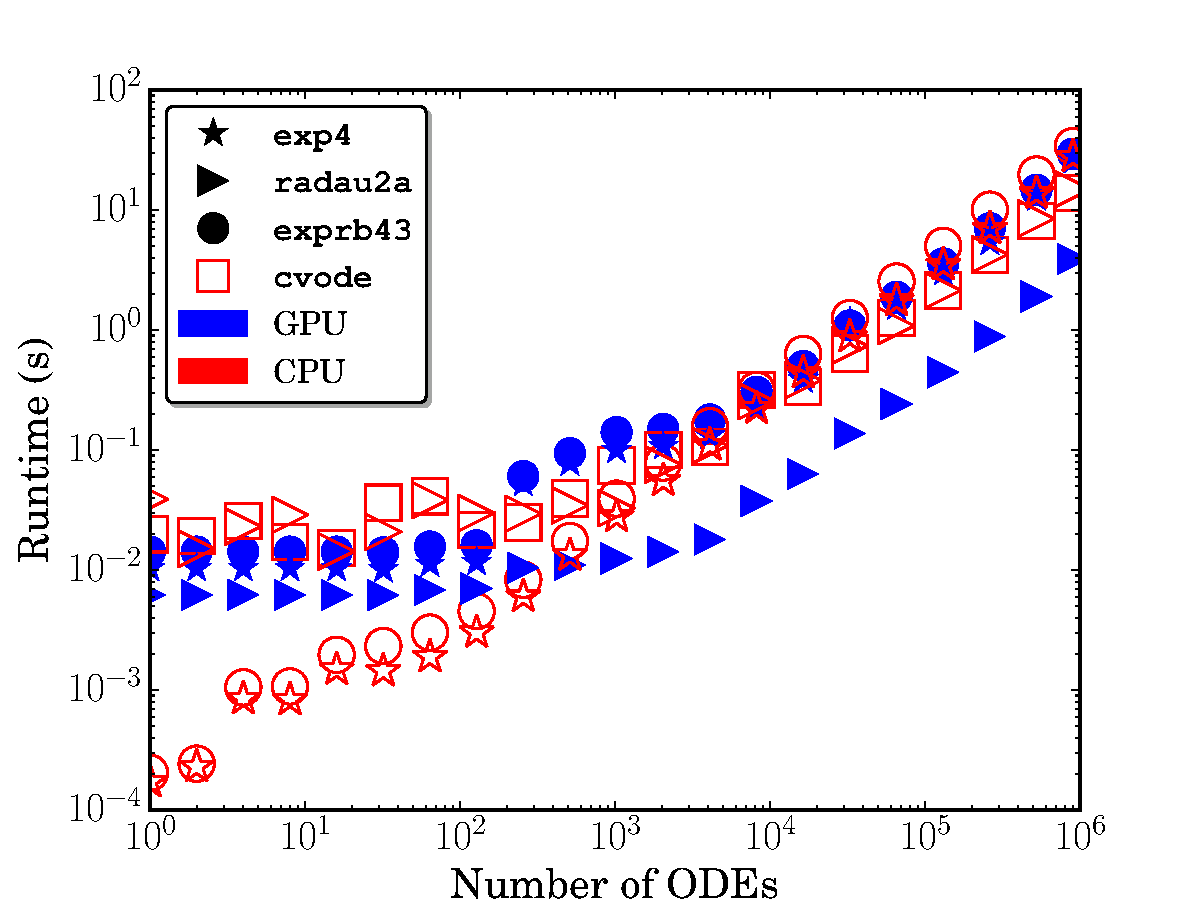
\includegraphics[width=\linewidth]{H2_1e-06_cpuvsgpu.pdf}
      \caption{$\delta t = \SI{1e-6}{\sec}$}
  \end{subfigure}
  \hfill
  \begin{subfigure}{0.48\textwidth}
      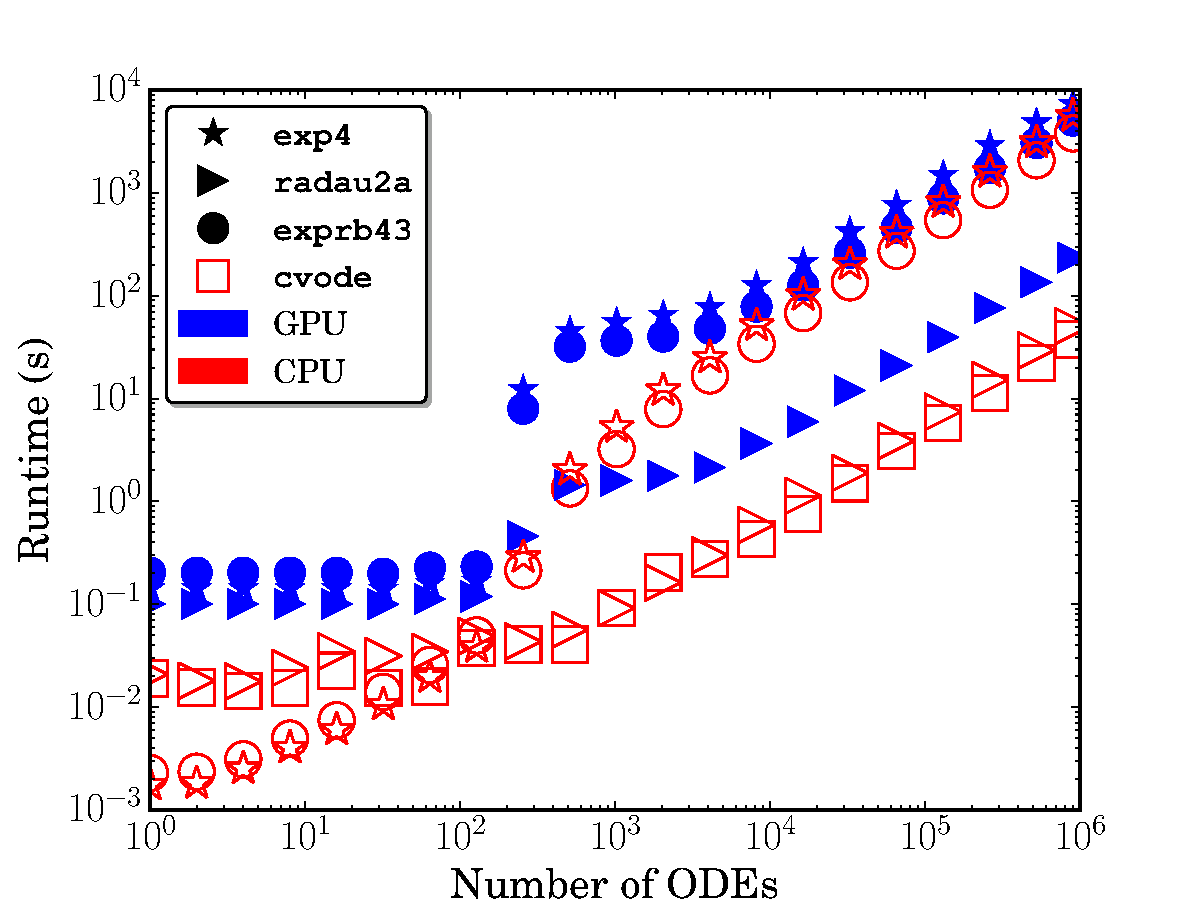
\includegraphics[width=\linewidth]{H2_1e-04_cpuvsgpu.pdf}
      \caption{$\delta t = \SI{1e-4}{\sec}$}
  \end{subfigure}
  \caption{Hydrogen}
  \label{F:H2_perf}
\end{figure}
\begin{figure}
  \centering
  \begin{subfigure}{0.48\textwidth}
      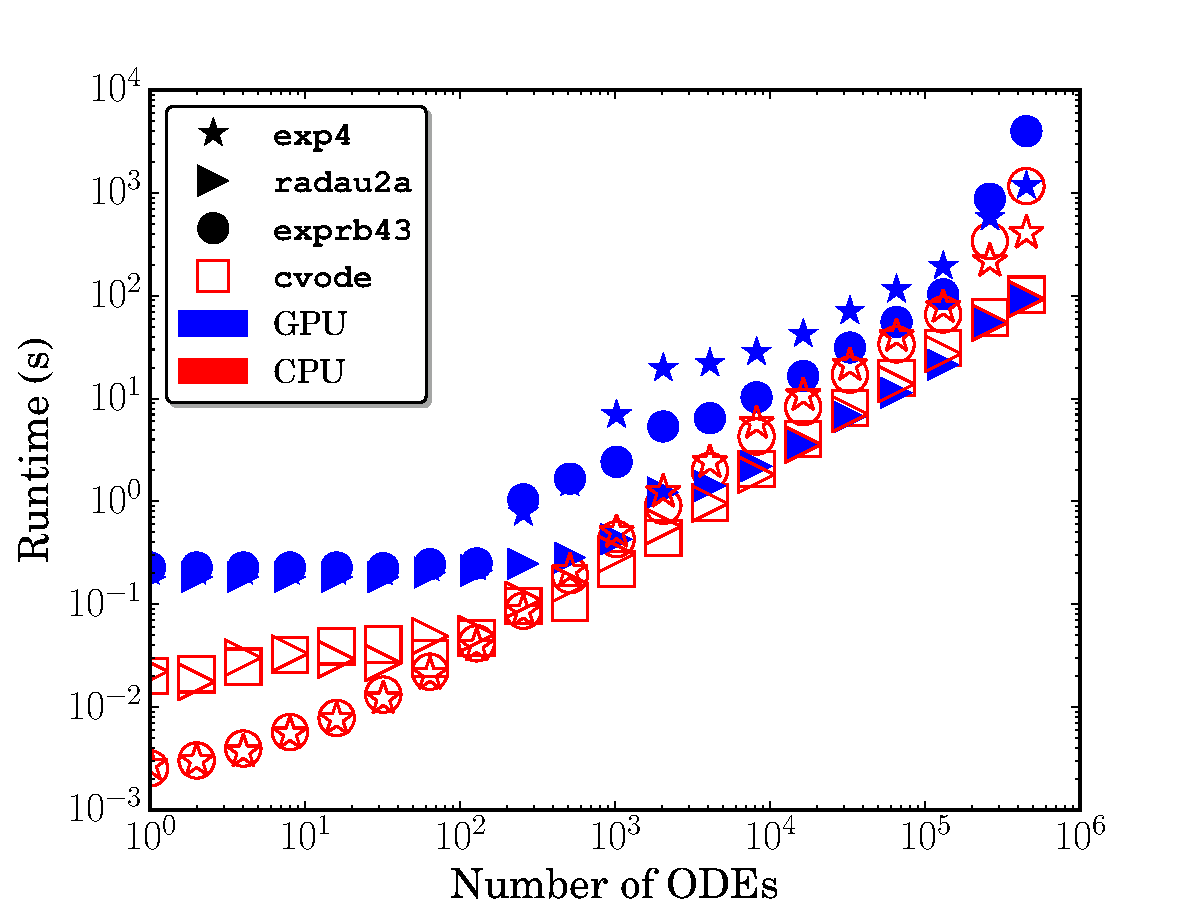
\includegraphics[width=\linewidth]{GRI_1e-06_cpuvsgpu.pdf}
      \caption{$\delta t = \SI{1e-6}{\sec}$}
  \end{subfigure}
  \hfill
  \begin{subfigure}{0.48\textwidth}
      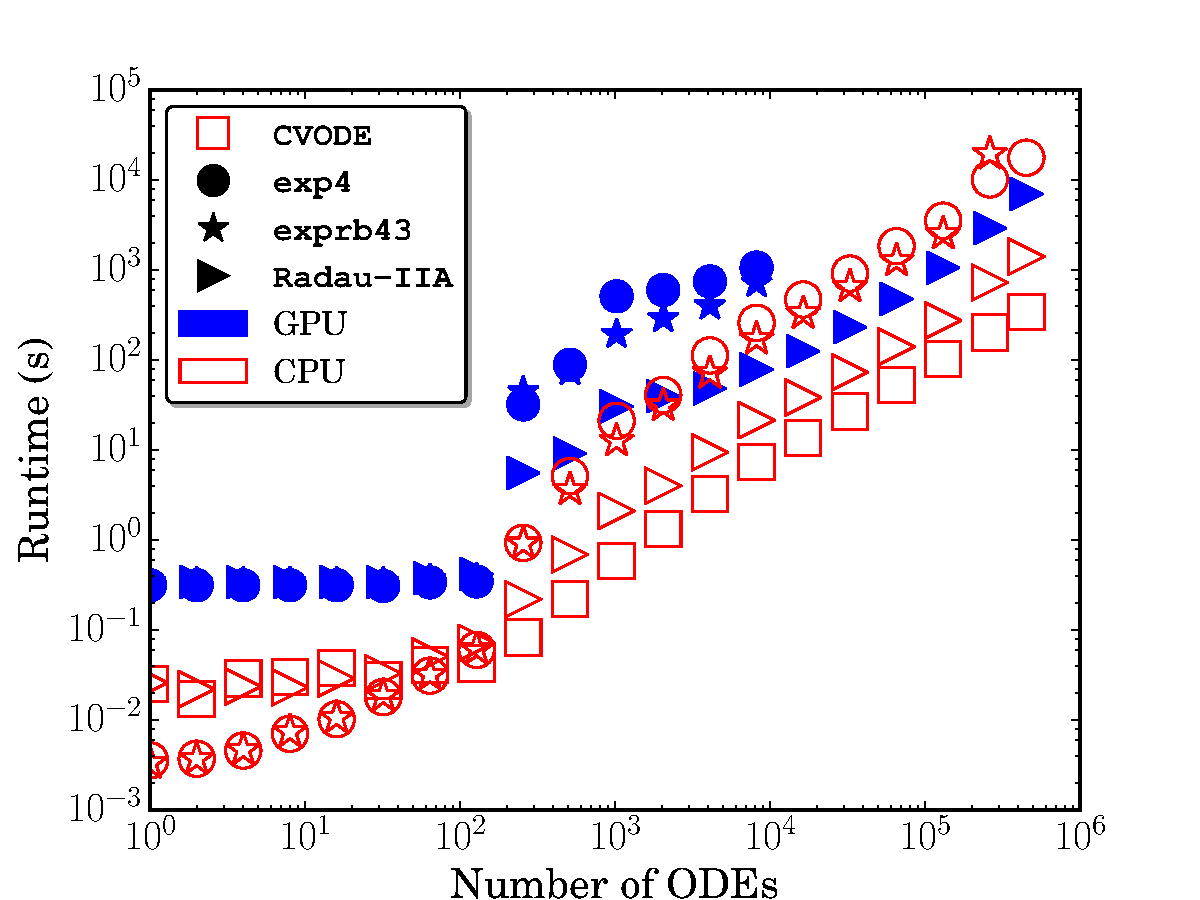
\includegraphics[width=\linewidth]{GRI_1e-04_cpuvsgpu.pdf}
      \caption{$\delta t = \SI{1e-4}{\sec}$}
  \end{subfigure}
  \caption{GRI}
  \label{F:GRI_perf}
\end{figure}
The performance of the integrators was tested on the PaSR conditions generated as described in Section~\ref{S:pasr} for two overall integration timesteps corresponding to representative timesteps of Large Eddy and Reynolds Averaged Navier Stokes simulations; $\delta t = \SI{1e-6}{\s}$ and $\delta t = \SI{1e-4}{\s}$ respectively.


\subsection{Limitations of the one ODE Per-Thread Approach}
During work on this paper, it was discovered that significant issues exist for the implementation of implicit and semi-implicit chemical-kinetic integrators on the GPU.
Namely, the size of the Jacobian itself places severe restrictions on either the maximum allowable mechanism size, or the total number of ODEs that can be solved concurrently.
For instance, the \texttt{Radau-IIA} solver requires storage of the Jacobian, as well as a LU factorized and a complex LU factorized matrix of the same size.
Similarly, the exponential integrators require storage of the Jacobian, the hessian matrix and vector subspace resulting from the Arnoldi process and the corresponding exponential of the hessian matrix.
While the hessian matrix, exponential hessian matrix, and vector subspaces can be smaller than the full Jacobian (e.g. by limiting the maximum Kyrlov subspace size), for the sake of simplicity in this analysis we shall assume they are full sized.
This implies that the storage requirements per ODE solved concurrently scales as $\mathcal{O}\left(3 \times N_s^2\right)$ for the \texttt{Radau-IIA} and at most $\mathcal{O}\left(4 \times N_s^2\right)$ for the exponential integrators, where $N_s$ is the number of species in the mechanism.

One method of storing these matricies (and other integrator variables) is in per-thread local memory.
This is advantageous from a programming standpoint, as it ensures coalesced memory access and simplifies indexing.
In CUDA however, all threads are limited to a maximum of \SI{512}{\kilo\byte} local memory, or \SI{64000}{\double} precision floating point numbers.
This limits the maximum mechanism size to relatively small numbers, as seen in Table~\ref{T:size_limits}.

Additionally, the Jacobian and associated matricies can be pre-allocated in global memory, and thus the total global memory is split between all threads in a given kernel launch.
In this work, a Tesla C2075 \todo{check} GPU was used, and similar models seem to be fairly typical for GPU based chemical kinetic integration studies, e.g. as in~\cite{Shi:2011aa,Niemeyer:2011aa,Shi:2012aa,Le2013596,Stone:2013aa,Niemeyer:2014aa}.
Assuming a reasonable launch configuration of \SI{64}{\threads} per block, with \SI{8}{\blocks} per streaming multiprocessor as on a C2050, we are limited to a maximum of $\sim\SI{4.19}{\mega\threads}$ (i.e. separate ODEs) per kernel launch.
For a \SI{6}{\giga\byte} global memory size, this works out to just \SI{178}{\doubles} available per thread.
Even assuming a more reasonable \SI{0.1}{\mega\threads}, or low \SI{0.01}{\mega\threads} per kernel launch, each thread is limited to just \SI{7500}{\doubles} and \SI{75000}{\doubles} correspondingly.
The resulting (approximate) maximum mechanism sizes are listed in Table~\ref{T:size_limits}.

In this study, even the USC mechanism with only 111 species caused the GPU to run out of local thread memory for all three GPU integrators.
As one potential benefit of GPU based integration algorithms is to allow use of larger, say 100--200 species, skeletal mechanisms in general reacting flow by acceleration of chemical kinetic integration compared to CPU integrators, these restrictive mechanism size limits pose a large issue.
It is noted that an chemical kinetic Jacobian based on species concentrations instead of species mass fractions is significantly more sparse~\cite{Lu:2009gh}, and thus may relax the mechanism size limits imposed by Jacobian storage.
This is an avenue that will be explored in future work.

\begin{table}[tbp]
\centering
\begin{tabular}{@{}l l l l@{}}
 \toprule
& \multicolumn{3}{c}{Mechanism Size Limit} \\
Memory Type & \texttt{Radau-IIA} & \texttt{exp4} & \texttt{exprb43} \\
\midrule
Local	    & 146 & 126 & 126 \\

Global (max)	    & 7 & 6 & 6 \\
Global (reasonable) & 50 & 43 & 43 \\
Global (low) & 158 & 136 & 136 \\
\bottomrule
\end{tabular}
\caption{
Approximate mechanism size limits for the various GPU integrators based on per-thread local memory limits, and global memory limits.
Max, reasonable and low refer to kernel launches with a total of \SI{4.19}{\mega\threads}, \SI{0.1}{\mega\threads} and \SI{0.01}{\mega\threads} respectively
}
\label{T:size_limits}
\end{table}

\pagebreak

\bibliography{refs}
\bibliographystyle{elsarticle-num}

\end{document}
